\begin{frame}
    \frametitle{NVIDIA Jetson Nano}
    \begin{columns}
        \begin{column}[]{0.5\textwidth}
            \begin{itemize}
                \item Runs Ubuntu
                \item Two camera ports (CSI)
                \item More powerful GPU than RPi
            \end{itemize}
        \end{column}

        \begin{column}[]{0.5\textwidth}
            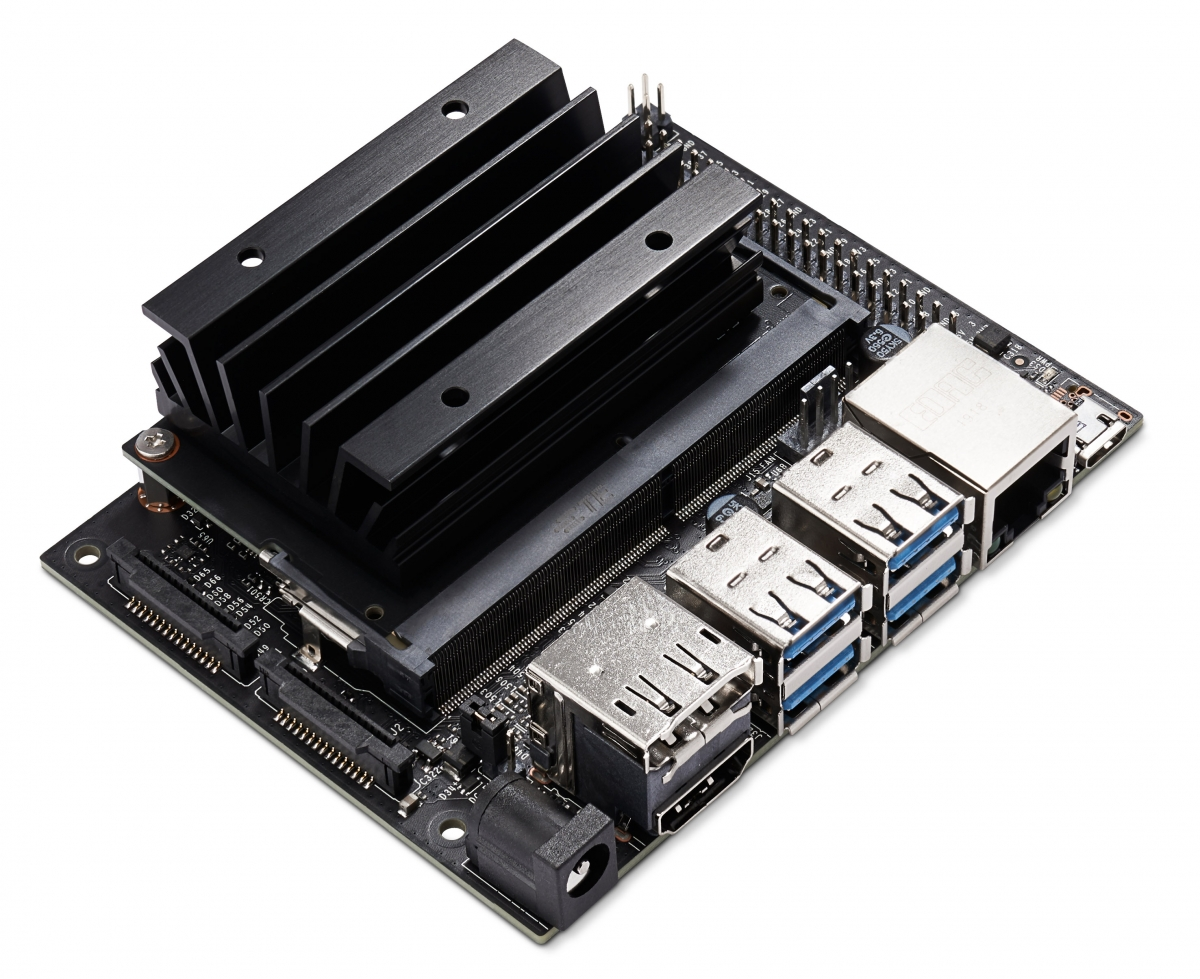
\includegraphics[width=\textwidth]{frames/img/nvidia.jpg}
        \end{column}
    \end{columns}


\end{frame}

\begin{frame}
    \frametitle{Cameras}
    \begin{columns}
        \begin{column}[]{0.5\textwidth}
            \begin{itemize}
                \item Compatible with NVIDIA and RPi
                \item Small package
                \item 8 megapixels
                \item Video:
                \begin{itemize}
                    \item 1080p @ 30 fps
                    \item 720p @ 60fps
                \end{itemize}

            \end{itemize}
        \end{column}

        \begin{column}[]{0.5\textwidth}
            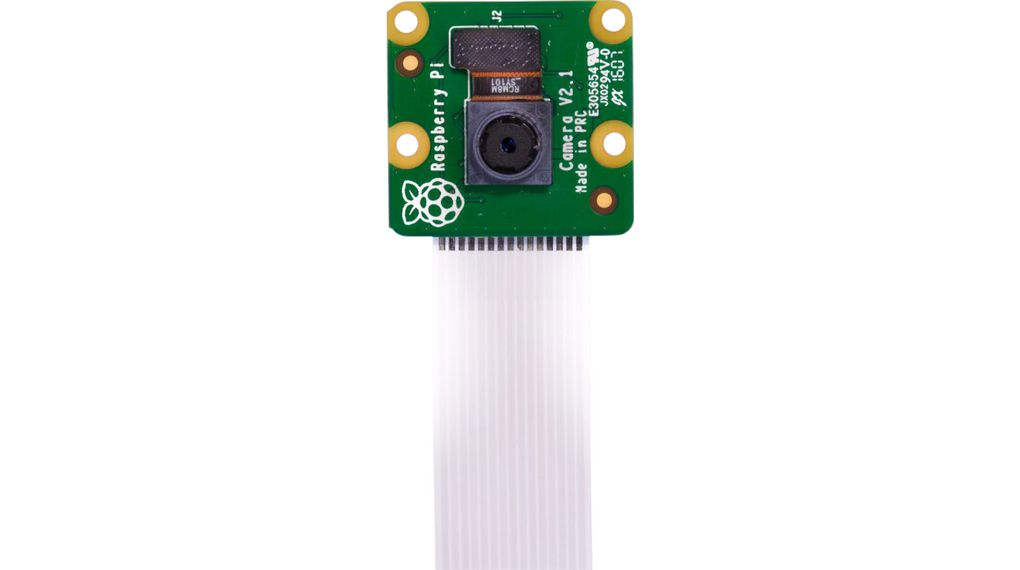
\includegraphics[width=\textwidth]{frames/img/camera.jpg}
        \end{column}
    \end{columns}
\end{frame}


\begin{frame}
    \frametitle{Dynamixel Smart Motors}
    \begin{columns}
        \begin{column}[]{0.5\textwidth}
            \begin{itemize}
                \item Connects in series
                \item Angle and wheel mode
                \item Feedback
            \end{itemize}
        \end{column}

        \begin{column}[]{0.5\textwidth}
            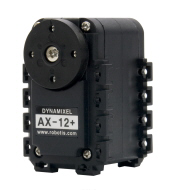
\includegraphics[width=\textwidth]{frames/img/dynamixel.png}
        \end{column}
    \end{columns}
\end{frame}

\begin{frame}
    \frametitle{Hardware}
    \centering
    \resizebox{7.0cm}{!}{
    \begin{tikzpicture}
        [align=center, node distance=1em, auto]

        \node [computing] (pc) {Arrowhead PC};
        \node [computing, below= of pc] (nvidia) {NVIDIA};
        \node [io, right= of nvidia] (battery) {Battery};
        \node [computing, right= of pc] (factory) {Factory};
        \node [io, below of= nvidia] (cameras) {Cameras};
        \node [io, right= 1em of cameras] (motors) {Motors};
        \node [io, left= 1em of cameras] (distance_sensors) {Distance sensors};
        \node [io, below= of motors] (arm) {Robot arm};
        \node [io, right= 1em of arm] (base) {Base};
        \node [rectangle=white, left= 5em of nvidia] (robot) {Robot};

        \path [line] (nvidia)--(cameras);
        \path [line] (battery)--(nvidia);
        \path [line] (battery)--(motors);
        \path [line] (nvidia)--(motors);
        \path [line] (nvidia)--(distance_sensors);
        \draw[->] (factory) -- (pc);
        \draw[<->] (pc) -- (nvidia);
        \draw[->] (motors) -- (arm);
        \draw[->] (motors) -- (base);
        \node [draw=black, dashed, fit= (nvidia) (battery) (distance_sensors)
        (cameras) (motors) (base) (arm)]{};

    \end{tikzpicture}
    }
\end{frame}

